\chapter{An Evolutionary View on the State of the Art}\label{ch:sota}

The goal of this chapter is to survey the development of the text generation from the old days until 2020. 

As conducted from the Introduction Chapter 1, Text Generation is the generic term for the output part of an automatic text summarizer. The research on Neural Text Generation and other fields had a major impact on the development of automatic text summarizers. In this chapter, I begin with the definition of a text generator in general and its historical development. I state out the most important steps from a basic text generator to a neural text generator. In the following I focus on the text summarizer and its personal historical evolution with the impacts of the neural text generators. There are several human-like summarizing state of the art technologies nowadays for the automatic text summarizers, but they are developed under a large scale data set and computional high demanding power. I am going to mention which parts are the fundamentals for my prototype and which technologies are state of the art, but not possible to achieve with a basic home computer.

\section{Structure of Text Generation }\label{ss:history}

Text Generation, Language modeling or Natural Language Generation are different words for basically the same meaning, but I will keep the denotation of Text Generation. A widely-cited survey from Reiter and Dale 1997 (Page 57-87) \cite{reiter} characterizes Text Generation as 'the sub-field of Artificial Intelligence and computational linguistics that is concerned with the construction of computer systems than can produce understandable texts in English or other human languages from some underlying non-linguistic representation of information' \cite{reiter}. This definition implies rather a data-to-text approach instead of the text-to-text approach from Table \ref{tab:nlp_table}, but in 1997 the rule-based approach dominated the neural end-to-end (Neural Text Generation) methods (Figure \ref{rules_based}). For that reason, in 2003 Evans declares Text Generation as quite difficult to define \cite{evans} (Page 144-151). Most researchers agree on text as the output synthesis part of the input-output system (e.g. Text Summarization or Image caption generation \cite{mitchell}). Whereas the input part can be not as easily distinguished \cite{mcdonald} (Page 191-197).

\subsection{Text Generation Tasks}

For the Text Generation input-output system, the system can be divided into six sub-problems \cite{reiter}. The following bullet points contain the six most crucial steps:

\begin{itemize}
	\item \textbf{Content determination}: Deciding which information to include in the text under construction
	\item \textbf{Text structuring}: Determining in which order information will be presented in the text
	\item \textbf{Sentence aggregation}: Deciding which information to present in individual sentences
	\item \textbf{Lexicalisation}: Finding the right words and phrases to express information
	\item \textbf{Referring expression generation}: Selecting the words and phrases to identify domain objects
	\item \textbf{Linguistic realization}: Combining all words and phrases into well-formed sentences
\end{itemize}

These six tasks can be though of an early decision processes. They suggest both a chronological order in which the tasks need to be solved, as well as an distinction between strategy and tactics. This distinction goes back to Thompson H. in 1977, where he first declared this two parts \cite{thompson}. Still, when it comes to modern neural state of the art Text Generation, the steps intersect in some ways. In the following comes a brief introduction to each of the steps. For the headline example is no aggregation necessary.

\subsubsection{Content Determination}

The first step is to determine which content should be present in the generated output text. Usually there is more information stored in the input than in the output. For this reason a certain \textit{choice} must be undertaken for the content. As mention in the case study (Section \ref{ss:case}, the headline can be summarized very precisely given only the first few sentences of the news. In this special case the determined content could be the first three sentences. For shorten a longer document into a summary, the key points need to be abstraced into a collection of preverbal messages and semantic representations of information, often expressed in the form of a logical or database like style \cite{gatt}. This means basically to group semtantical similar words and phrases together, to remove redundancies. This step followed for the most time a rule-based approach, but in recent years researchers developed a data-driven approach (more in Section \ref{ss:archi}). For example, Barzilay and Lee (2004) developed a method to determine the content through Hidden Markov Models (HMM) \cite{lee} (Pages 113-120). Hidden Markow Models are stochastical models named after the russian mathematician A. A. Markow. They chain up different states of a system, in our case different topics of one or many news articles. This topics automatically will be clustered together as sentences based on the natural language semantical meaning \cite{gatt}. 

\subsubsection{Text structuring}

After successfully deciding which contents will be used in the generated text, the structure or order of this fragments need to be determind. Given the example article from Table \ref{tab:google}:

\begin{tcolorbox}
\begin{center}
		Australian wine exports hit a record 52.1 million liters worth 260 million dollars (143 million us) in september, the government statistics office reported on monday 
\end{center}
\end{tcolorbox}

A good news headline should give all necessary information for the reader, namely:

\begin{itemize}
	\item Where did it happen? -> \textit{Australia}
	\item What happened? -> \textit{Wine exports, record high}
	\item Who did something? -> \textit{Australia}
	\item When did it happen? -> \textit{September}
\end{itemize}

For our example the content was already predefined in the first step, now the important words and sentences will be reorder based on this four questions. Generalization approaches for the ordering task have already been proposed. Lapatas approach \cite{lapata} (Page 471-484) tries to find an optimal ordering of \textit{information-bearing-items}. This method can even be applied to multi document input, which is more difficult to solve than single document inputs (explained in Section \ref{ss:multidoc}).

\subsubsection{Sentence aggregation}

By combining separate sentences with similar meaning into one, the generated text becomes potentially more fluid and enhances the readability \cite{dal} (Pages 383-414) \cite{cheng-mellish2000} (Pages 183-193). For example, an aggregation makes sense for a football games and its results published in the Google News. Google could web scrape the live tickers of goals and after collecting all the data a possible result would be:

\begin{tcolorbox}
	\begin{center}
		(1) Mario Götze scored after 19 minutes and 23 seconds \\
		(2) Mario Götze scored after 20 minutes and 30 seconds \\
		(3) Mario Götze scored after 60 minutes and 11 seconds
	\end{center}
\end{tcolorbox}

This is obviously not redundant, because it contains new information in every sentence, but for summarizing it, the sentences can be aggregates into:

\begin{tcolorbox}
	\begin{center}
		(4) Mario Götze scored 3 times within 51 minutes
	\end{center}
\end{tcolorbox}

Aggregation is not an easy task, because it is not intuitive for an algorithm to detect semantic similarities and at the same time new information in that. Furthermore it depends highly on the to achieving output which kind of aggregation the text should undergo. A general approach was proposed by White and Howcraft (2015). They designed an algorithm to detect parallel verb phrases (\textit{scored after}) in multiple (three) sentences and elide the subject and the verb in the generated sentence \cite{white-howcroft-2015-inducing} (Pages 28-37). 

\subsubsection{Lexicalisation}

After the sentences have been aggregated and finalized, the next step is lexicalisation, which converts the sentences into natural language. A single event can be expressed by natural language in multiple ways. For example the scoring event from the last section could be expressed as \textit{scored three goals} or \textit{goaled for three times}. The complexity for the lexicalisation step correlates with the amount of alternative sentences available. Furthermore it is important if there summary is limited with an amount of variation \cite{Theune} (Pages 47-86). Whether or not the text shall be processed with lexical variation in its generated sentences or not depends on the application field. In needs to be decided in advance. For example the soccer game is more likely to be converted into a different styles than a weather forecast. Another important difficulty is to design the way on how the lexicalisation cares about gradable properties. For example if the liveticker was:

\begin{tcolorbox}
	\begin{center}
		(1) Mario Götze scored fast after 3 minutes and 23 seconds
	\end{center}
\end{tcolorbox}

Then the systems needs to know whether the football player scored fast in a way that it is an early stage of the game, or he ran in such a fast way and scored with the pace. Humans tend to perceive different, as Power and Williams (2014) pointed out in an evaluation. A timestamp expression of \textit{00:00} can be perceived as \textit{midnight}, \textit{late evening} or simply even \textit{evening} for some people \cite{Power} (Pages 113-134).


\subsubsection{Referring expression}

Referring Expression Generation is highly characterized by Dale and Reiter in 1997. They came up with the idea to identify words and phrases as domain entities. Nowadays this is also known as \textit{Named Entity Recognition}. This step shows some similarity to lexicalisation, but Dale and Reiter pointed out that expression referring is \textit{a discrimination task, where the system needs to communicate sufficient information to distinguish one domain entity from other domain entities} \cite{reiter2}. From the previous example, \textit{Mario Götze} can be denoted with his name, another way would be calling him \textit{football professional} or \textit{the athlete}. Many factors play a role in how to determine which expressions and factors play a role in a particular context. Referring expression generation can basically be broken down into two steps.
The first step is to decide the shape of referring expression. What type of reference should be used (e.g., a proper name or described with his/her job) \cite{named}. The second is to determine the content of the referring expression (e.g., Mario Götze or the athlete) \cite{named}.
Rule-based approaches as well as the state of the art Machine Learning approaches have been proposed to solve this task \cite{reiter2}.  

The usual limitation of previous referring expression generation systems is that they are not able to generate referring expressions for new, unseen entities \cite{anja} (Pages 294-327). With the use of modern Machine Learning approaches, this limitation has overcome.
\subsubsection{Linguistic realisation}


\subsection{Architectures and Approaches}\label{ss:archi}


nlg-survey-long Kapitel 3

\begin{itemize}
	\item Rule-based, modular approaches
	\item Planning-based approaches
	\item Data-driven approaches
\end{itemize}

\subsubsection{Rule-based approach}
\subsubsection{Planning-based approach}
\subsubsection{Data-driven approach}




\section{Advanced Approaches for Text Generation}
\subsection{Recurrent Neural Networks}
Even though I introduced the neuron in a neural network as a kind of brain cell imitation, the neuron of a basic neural network will forget everything when it is shut down, unlike the brain. Making information persistent is a crucial step towards better performing models. Recurrent neural networks, or RNN, address this issue. They are networks with integrated loops, which allow the information to persist \cite{olah}. The network architecture of the RNN is important, because it denotes the first step into neural text generation and neural text summarization. 

\begin{figure}
	\begin{center}
		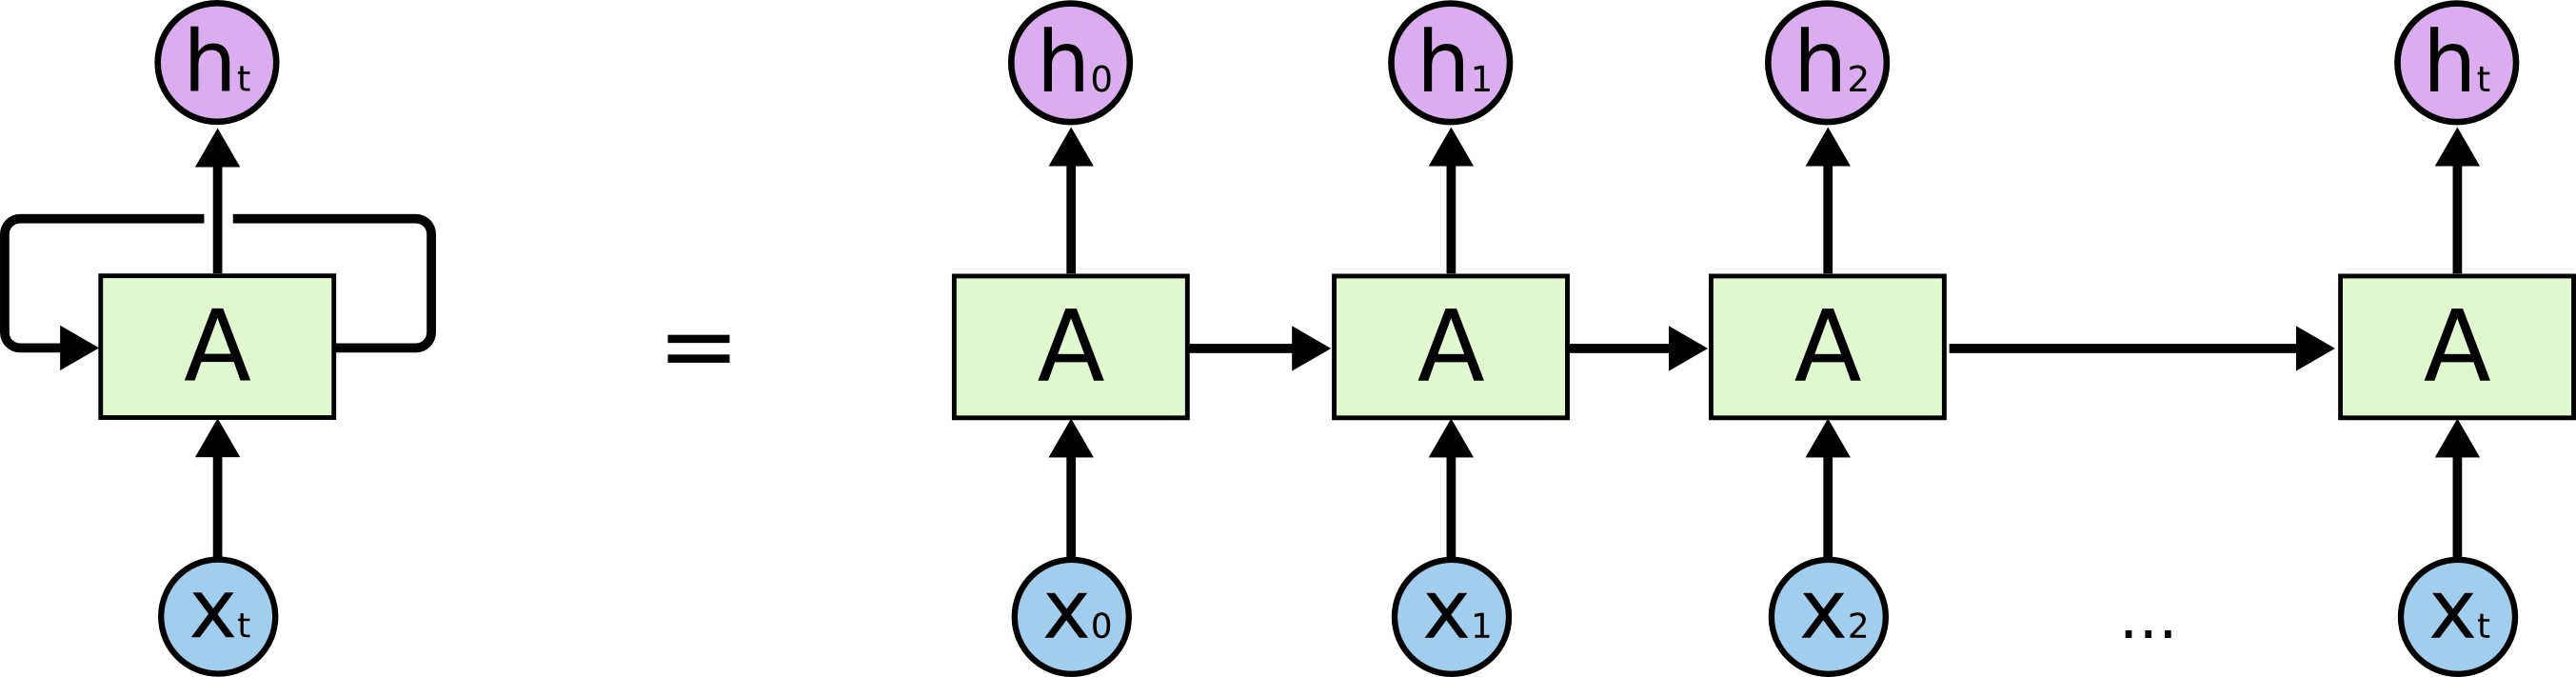
\includegraphics[width=4.5in]{photos/RNN-unrolled}\\
		\caption{Recurrent Neural Network with integrated loops \cite{olah}}\label{rnn}
	\end{center}
\end{figure}

Figure \ref{rnn} shows an unrolled Recurrent Neural Network. The input \(x_t\) on time step \textit{t}, is passed to the neural network \textit{A}. The network looks at the input on this time step and outputs the hidden state \(h_t\) at the same time step \textit{t}. This loop allows the network to pass information from one time step to another. The picture \ref{rnn} shows, that the learned parameter from input \textins{x} on time step \textins{t} will be passed as additional information to the next time step \textins{t + 1} and so on. For example if a RNN wants to predict the next word in the sentence "Since I am living in Hong Kong .. by now I speak fluent \textit{Cantonese}". The network needs to remember that the target country is Hong Kong to predict the language Cantonese. At each time step \textit{t}, the hidden state \textit{\(h_t\)} of the Recurrent Neural Network is updated by:

\begin{center}
\begin{math}
\boldsymbol{h_{(t)}} = f(\boldsymbol{h_{(t-1)}}, x_{t})
\end{math}
\end{center}

where \(f\) is a non-linear activation function and \textit{x} is the input in form of a word. The function \(f\) can be in the simplest case a sigmoid function which has either 0 or 1 as output, or the more complex and effective Long Short Term Memory cell, explained in the next Section \ref{ss:lstm} \cite{hochreiter1997long}. The Recurrent Neural Network is trained to predict for example the next word in a sentence or sequence. This prediction is possible due of the learned probability distribution over a sequence. The output at each time step \textit{t} is a conditional distribution \(p(x_{t}|x_{t-1},...,x_{1})\).

Theoretically with this approach it is possible to retain information from many time steps ago, but unfortunately, as the time span back grows, RNN's become unable to learn the information from too long ago cells. This phenomenon was explained by Sepp Hochreiter in 1991 \cite{Hochreiter:91} under the name \textit{vanishing gradient problem}. The solution to this problem is the Long Short Term Memory, short LSTM.

\subsection{Long Short Term Memory}\label{ss:lstm}
Long Short Term Memory cells were first proposed by Sepp Hochreiter and Jürgen Schmidhuber in 1997 \cite{hochreiter1997long}. The LSTM is a special kind of Recurrent Neural Network, because it is able to remember long-term dependencies and informatiom. The goal of the cell is to solve the vanishing gradient problem of the Recurrent Neural Network. Inputs into this cell can be stored for a long period of time, without forgetting them, as in Recurrent Neural Networks. The LSTM is designed to avoid the loss of information (vanishing gradient problem), by intentionally ledging on to certain information over plenty of time steps. 

\begin{figure}
	\begin{center}
		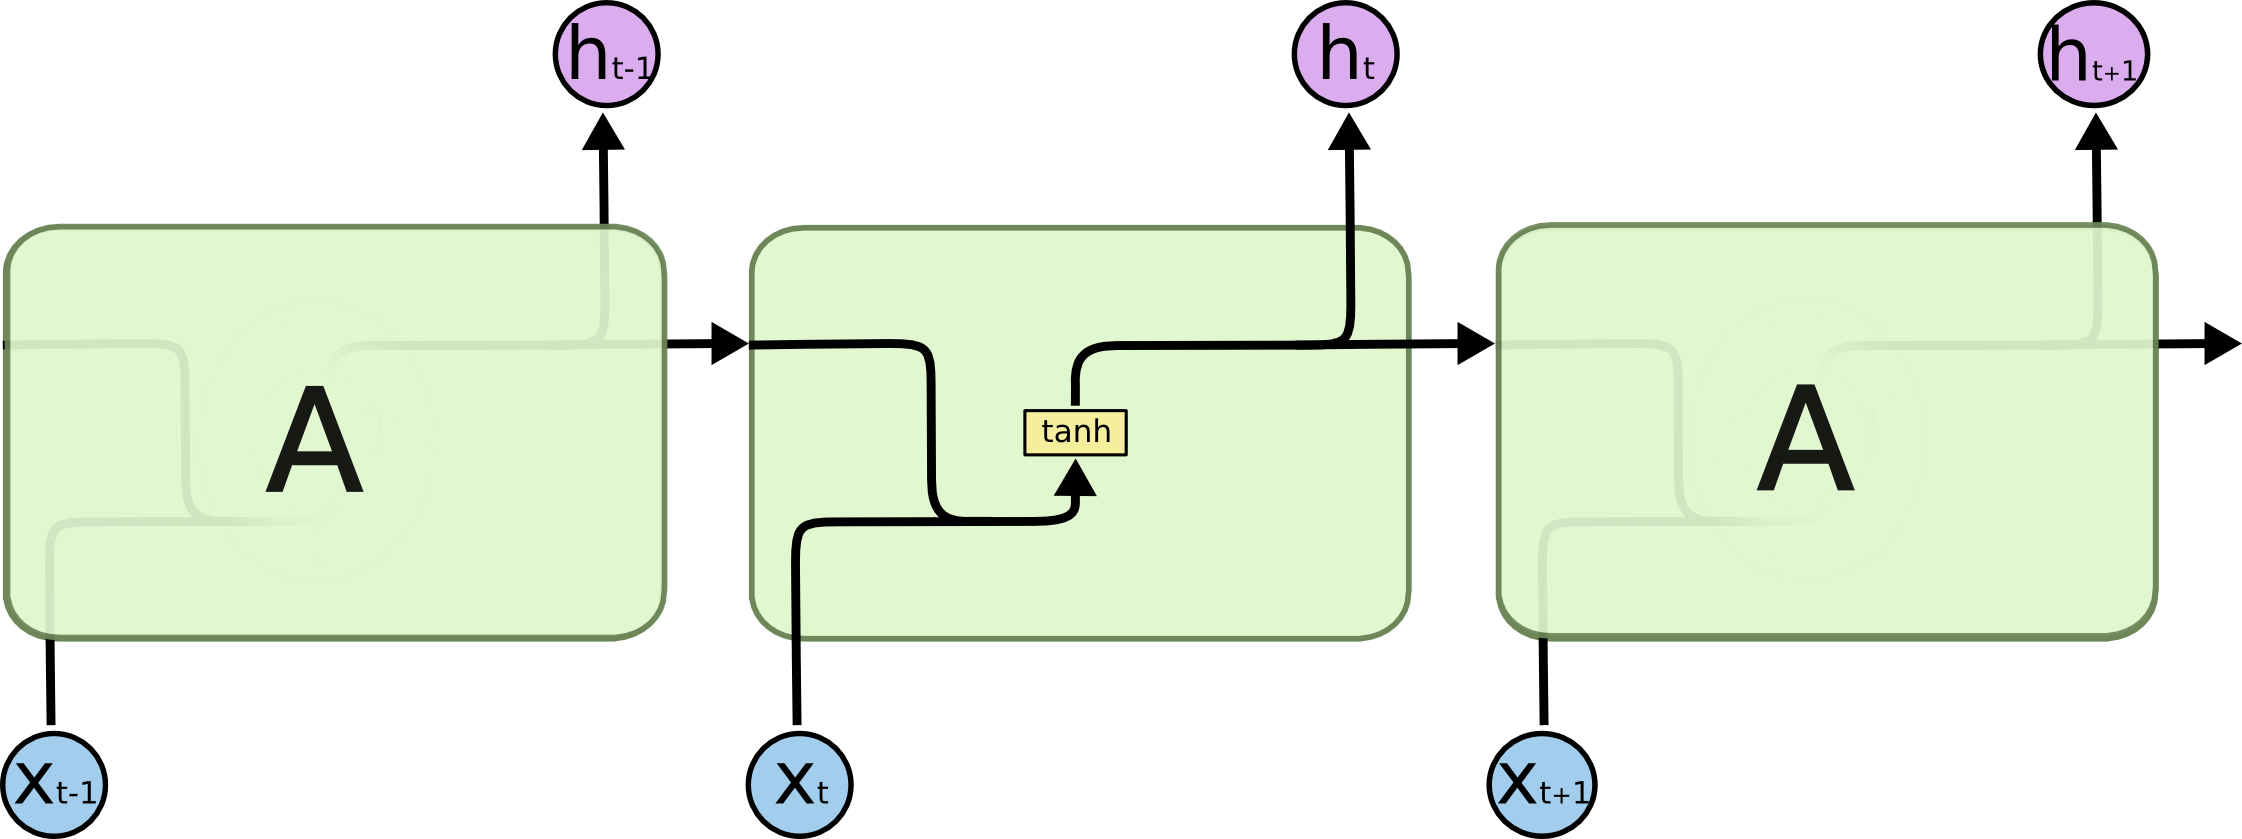
\includegraphics[width=4.5in]{photos/LSTM3-SimpleRNN}\\
		\caption{The repeating module in an Recurrent Neural Network contains one single layer \cite{olah}}\label{lstm}
	\end{center}
\end{figure}

LSTM's can be enrolled the same way like RNN's, but there is a core difference between the Recurrent Neural Network in Figure \ref{lstm} and the Long Short Term Memory in Figure \ref{lstm2}. The LSTM has four gates instead of one like the RNN. The four gates are:

\begin{itemize}		
	\item Forget Gate
	\item Input Gate
	\item Cell State
	\item Output Gate
\end{itemize}

\begin{figure}
	\begin{center}
		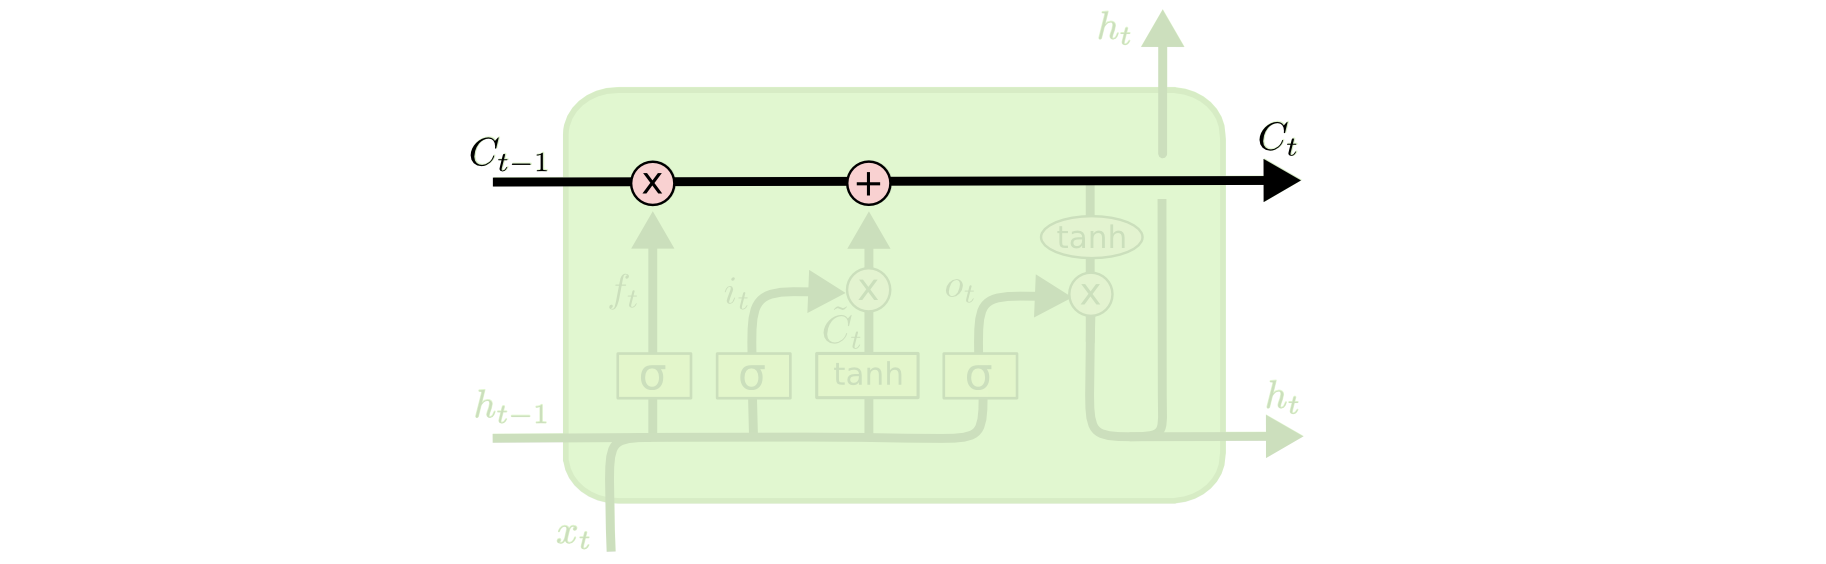
\includegraphics[width=4.5in]{photos/LSTM3-C-line}\\
		\caption{Cell State of the Long Short Term Memory which acts as data highway \cite{olah}}\label{lstm3}
	\end{center}
\end{figure}

The \textbf{Forget Gate} decides what information should be thrown away or kept. Information from the previous hidden state and information from the current input is passed through a sigmoid function. A sigmoid function takes an input and returns high values closer to 1 and smaller values closer to 0. The closer to 0 means to forget the state, and the closer to 1 means to keep the state.

The \textbf{Input Gate} updates the cell state. That decides which values will be updated by computing the values to be between 0 and 1 like the Forget Gate. Important information is closer to 1 and 0 means less important.

The \textbf{Cell State} is the core of the LSTM. It is the horizontal line shown in Figure \ref{lstm3}. The cell state acts like the information highway in the cell. With only some minor linear computation, it runs through the entire cell. This way information can pass very easily through the cell. 

The \textbf{Output Gate} decides what the hidden state of the next LSTM cell should be. The hidden state contains information on previous inputs and it is also used for predictions. The hidden state denotes the state which is passed from the output gate on time step \textit{t} to the input gate for the LSTM cell on time step \textit{t+1}.


\begin{figure}
	\begin{center}
		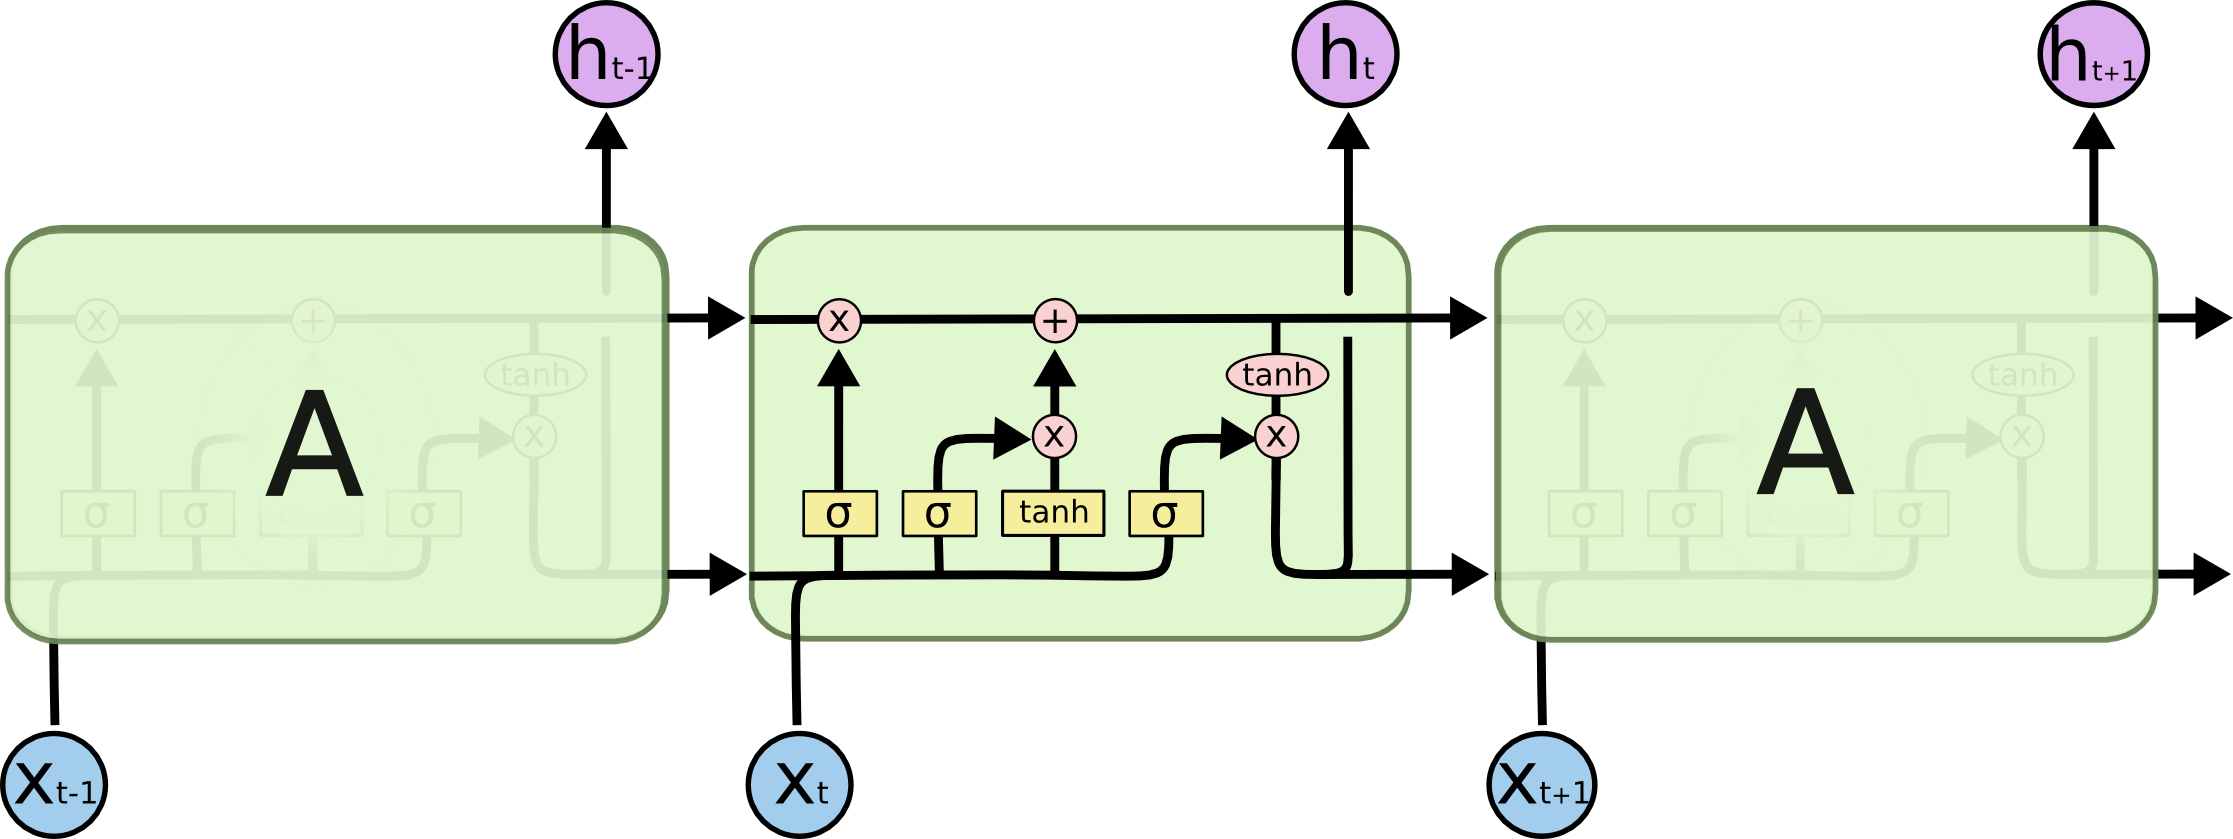
\includegraphics[width=4.5in]{photos/LSTM3-chain}\\
		\caption{The repeating module in an LSTM contains four interacting layers \cite{olah}}\label{lstm2}
	\end{center}
\end{figure}

The main idea of the LSTM is, that it can decide which information to remove, to forget, which to store and when to use it. It can also decide when to move the previous state information to the next, like the RNN shown in Figure \ref{rnn}. Even though many variations of the LSTM occupy the state of the art performance, the LSTM is used in many real business cases in production, like the Google translater or weather forecasting.
The Long Short Term Memory paved the way for the sequence to sequence models.
\subsubsection{N-Grams}\label{ss:ngram}

\subsection{Sequence to Sequence}\label{ss:seq2seq}
In the year 2014, Google invented a new way to translate language by learning a statistical model with a neural machine translation approach \cite{seq2seq}. Google called it Sequence to Sequence model \cite{seq2seq}, often shortened down to seq2seq, which consists of an encoder and a decoder. 

Before that, language translation was originally processed by rule-based systems \cite{chen-goodman}. The systems computed their work by breaking down sentences into plenty of chunks and translating them phrase-by-phrase, but this approach created not easily understandable language.

After rule-based systems, statistical models have taken over the. Given a source text in e.g. German (\textit{f}), what is the most suitable translation into e.g. English (\textit{e})? The statistical model p(\textit{g}|\textit{e}) is trained on multiple texts (corpus) and finally outputs p(\textit{e}), which is calculated only on the target corpus in English. 

\begin{center}
\begin{math}
\hat{e} = argmax_{e}(e|g) = argmax_{e} p(g|e) p(e)
\label{eq:rule}
\end{math}
\end{center}

The formula means, among all Baysian probabilities p(\textit{g}|\textit{e})p(\textit{e}), select the pair of words (translation), select the most likely to be the best translation (argmax). Even though this approach produces good results, it looses the wider semantical view, and so it is especially not effective for a good summarization technique.

For the first time, neural networks in form of feed-forward fully-connected neural networks produced such good results, that they replaced all non-network techniques. Affine matrix transformations are stacked together and are followed by non-linearities to the input and each following hidden layer \cite{Bengio} Page 1141-1142. However, these models require a fixed content length for their calculations, which makes them again not flexible enough to produce human-like translations. 

Even if a LSTM (Section \ref{ss:lstm}) was used to map sequences of words from one language to another, it will most likely produce errors or bad results. A single LSTM cell needs the same input length and output length, which is unrealistic for translating multilingual. For example the English "He is running" translated into German is "Er rennt". The LSTM itself can not translate that, because of the different word length. 
The Long Short Term Memory cell from Section \ref{ss:req} was invented independently from the sequence to sequence models, but
finally three employees of Google published a paper about their approach to make use of the LSTM to create a sequence to sequence model, also called encoder-decoder model.
The basic idea is that the encoder converts an input text to a latent vector of length \text{N} and the decoder generates an output vector of length \textit{V} by using the latent encoded vector. It is called a latent vector, because it is not accessible during the training time (manipulating it), for example in a normal Feed Forward Neural Network, the output of a hidden layer in the network can not be manipulated. The initial use of encoder-decoder models was for machine translation.

Technologies for a specific field in the machine learning environment and especially text generation can often be used cross functional. The encoder-decoder model found its way into text summarization and automated email reply by Google \cite{google} as well. Figure \ref{enc-dec} illustrates the model for Google's automated email reply.

\begin{figure}
	\begin{center}
		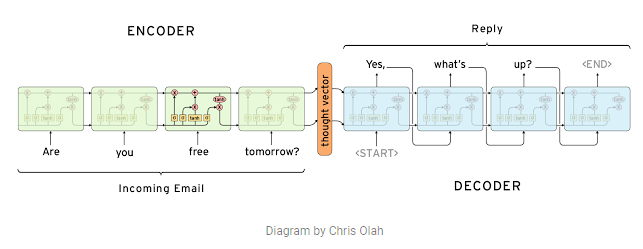
\includegraphics[width=5.5in]{photos/encoder_decoder}\\
		\caption{LSTM encoder-decoder model for automated E-Mail reply}\label{enc-dec}
	\end{center}
\end{figure}

Figure \ref{enc-dec} makes use of an Long Short Term Memory cell, which captures situations, writing styles and tones. The network generalizes more flexible and accurate than a rule-based model ever could \cite{google}. 


\subsection{Encoder and Decoder}

In the following, the encoder and then the decoder will be explained to have a better insight in how this technology works. The prototype from Chapter \ref{ch:proto} is based on this kind of model. As already mentioned a sequence to sequence model is often referred to as a encoder-decoder model. The sequence to sequence model itself is built using a Recurrent Neural Network or a Long Short Term Memory as explained in the last Section \ref{ss:seq2seq}.

\begin{figure}
	\begin{center}
		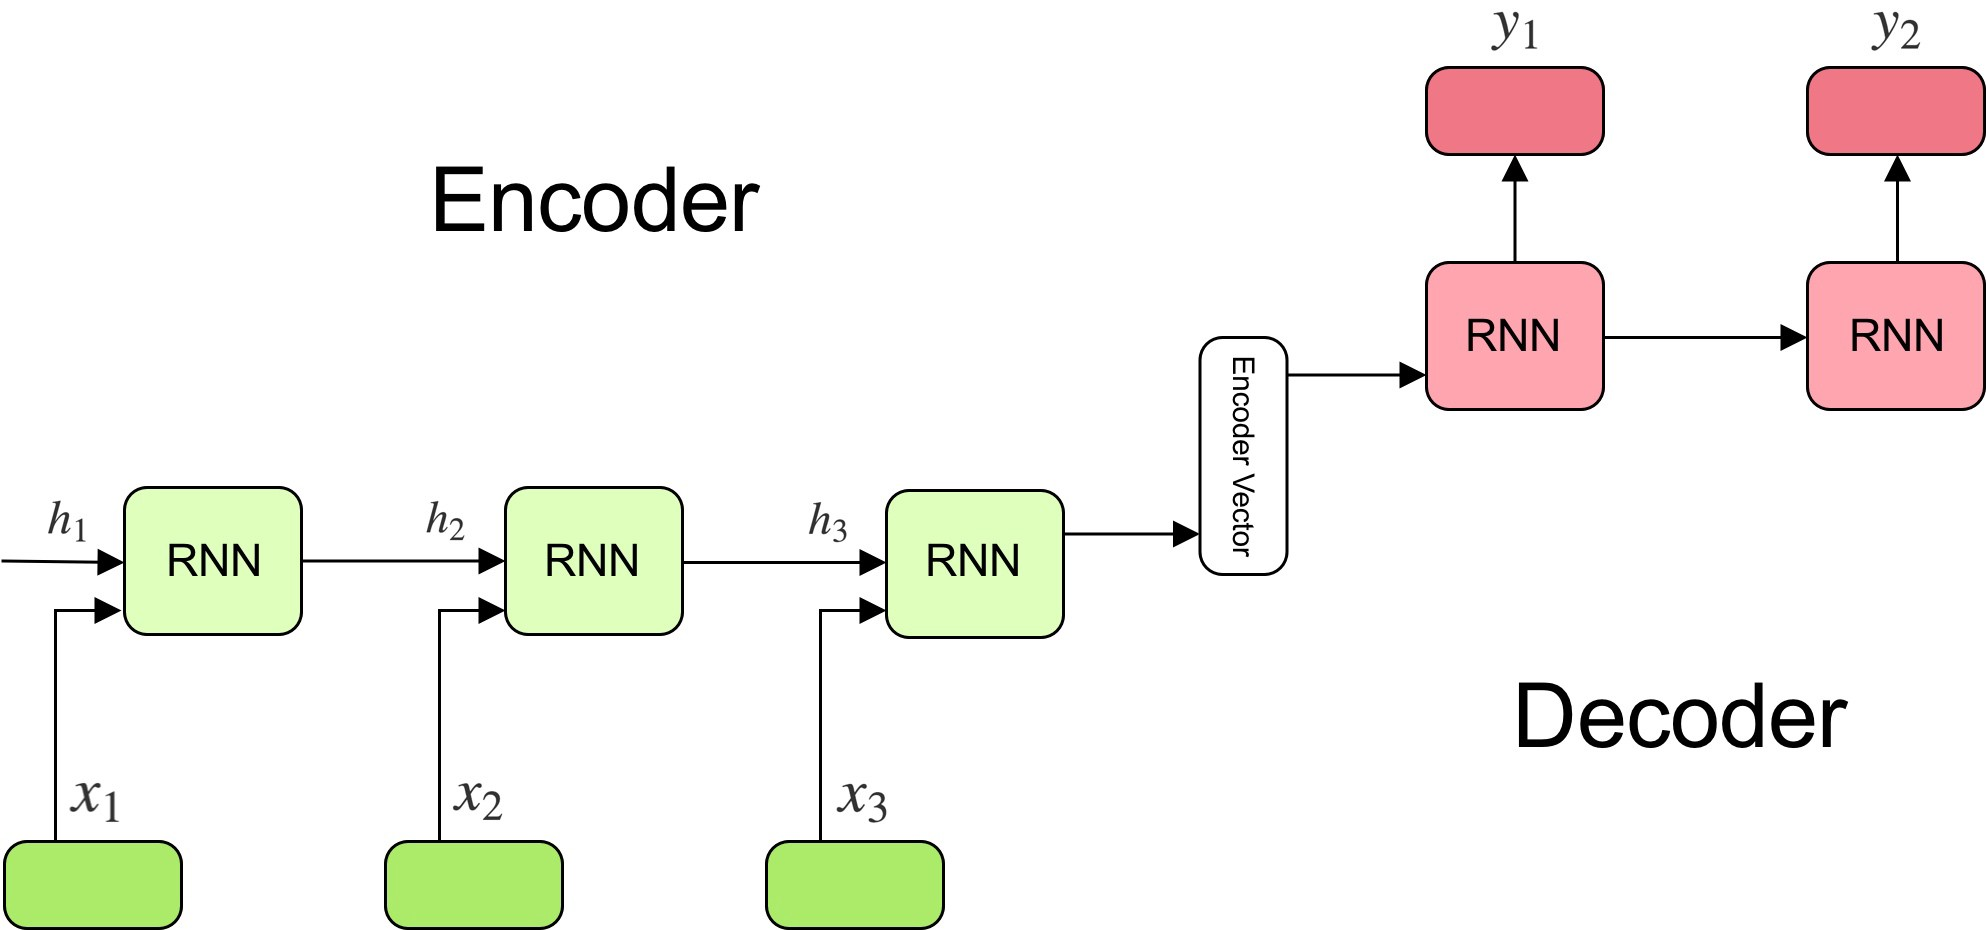
\includegraphics[width=4.5in]{photos/encoderdecoder.jpeg}\\
		\caption{Encoder-decoder sequence to sequence model \cite{encdec}}\label{encdecseq}
	\end{center}
\end{figure}

Figure \ref{encdecseq} shows, that the encoder decoder model is built up from actually three parts:

\begin{itemize}
	\item Encoder
	\item Intermediate (encoder) Vector
	\item Decoder
\end{itemize}


The \textbf{Encoder} iteratively integrates the words in a sentence into the hidden state \textit{h} into the Long Short Term Memory cell.
Figure \ref{lstm3} shows a single LSTM cell with the input cell state \textit{C} at the time step \textit{t-1}  and the input of the hidden state \textit{h} at the same time step \textit{t-1}. This is necessary for the cell to compute both the input words, but also the knowledge from prior words. Words are represented as latent vectors in the sequence to sequence models and are stored in a vocabulary table. Each fixed length vector stands for a word in the vocabulary, for example the vector length is fixed to a dimension of 300. In a simple case, the number of words in the vocabulary is fixed to e.g. 50.000 words, hence the dimension of the vocabulary table in Figure \ref{voctable} is [50000 x 300]. 

\begin{figure}
	\begin{center}
		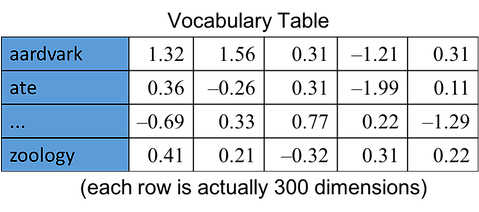
\includegraphics[width=3.5in]{photos/w1-16}\\
		\caption{Snippet of an example vocabulary table \cite{mugan}}\label{voctable}
	\end{center}
\end{figure}

A connection of multiple recurrent units (three in Figure \ref{encdecseq}) where each accept a single element as an input, gains information and propagates it forward to the next cell and accordingly the next time step. In the example of Figure \ref{encdecseq}, the hidden state of \textit{h3} is calculated based on the prior two cells.


The \textbf{Encoder Vector} is the last hidden state of all the encoder cells, in this example the encoder vector is located at the output of cell three. The vector tries to combine all of the information from the prior encoded words with the purpose to help the decoder make accurate predictions. Basically, the encoder vector is the initial input for the decoder part of the model.

The \textbf{Decoder} unrolls the encoder vector from meaning space into a target sentence. The meaning space (shown in Figure \ref{meaningspace}) is a mapping of concepts and ideas that we may want to express to points in a continuous, high-dimensional grid \cite{mugan}. 
The minimum requirement for the meaning space is to consist at least of the last state of the encoder Recurrent Neural Network (encoder vector). The decoder computes a probability distribution for each word in the encoder vector to generate the next state. In the example case, the output is generated by multiplying the hidden state in the encoder vector \textit{h} by the output matrix of size [300 x 50000]. The product of this matrix multiplication is a vector of size [50,000], that can be normalized with a \textit{softmax} into a probability distribution over words in the vocabulary. The network can then choose the word with the highest probability, because the softmax squeeses all outputs into a summed up probability of 1. For example:

\begin{tcolorbox}
	"Since I am living in Hong Kong, by now I speak fluent ... "
	
	\begin{itemize}
		\item Cat: 0.01
		\item running: 0.005
		\item Cantonese: \textbf{0.5}
		\item Mandarin: 0.3
		\item French: 0.015
	\end{itemize}

	The chosen word is \textbf{Cantonese}, because it is the highest probability among all probabilities which are summed up to 100\%
\end{tcolorbox}
 

\subsection{Attention}
In general, the explanation of the sequence to sequence models just covered the very basic idea of the model. To achieve the state-of-the-art result, not only a single vector can be used for encoding the entire input sequence, but multiple vectors each capable of capturing other information. 

\begin{figure}
	\begin{center}
		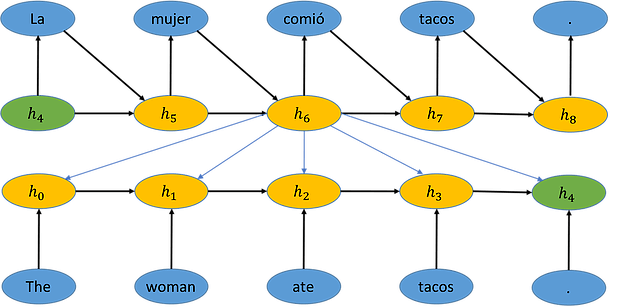
\includegraphics[width=4.5in]{photos/w1-11}\\
		\caption{Attention mechanism for Spanish-English translation \cite{mugan}}\label{attention1}
	\end{center}
\end{figure}
In the encoder and decoder model, the length of the state vector \textit{h} does not change for the input and output. As shown in the example of Section \ref{ss:seq2seq}, sentences translated into another language can have a different word length. For the model to automatically adjust the length of the output, is to use the technology called \textit{attention} \cite{attention} \cite{attention2}.

Figure \ref{attention1} shows the basic concept of attention. The Long Short Term Memory is not starting to right before time step \textit{t = 6} at state \textit{\(h_{6}\)}. Attention enables the network to look at all prior encoded states of the words, takes the weighted average probability of the vectors and also uses this as additional information. Attention also projects its vectors into the meaning space (Figure \ref{meaningspace}. 

\begin{figure}
	\begin{center}
		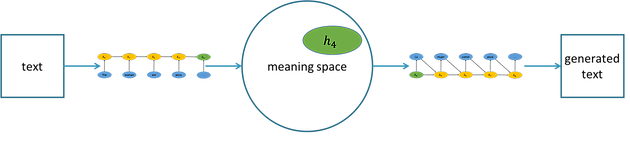
\includegraphics[width=3.5in]{photos/w1-21}\\
		\caption{Meaning Space of the Attention model \cite{mugan}}\label{meaningspace}
	\end{center}
\end{figure}

Sequence to sequence models can be entirely built up from the attention model \cite{attention2}. 

\section{Structure of Text Summarization}

In the modern era of big data, retrieving useful information from a large number of textual documents is a challenging task due to the unprecedented growth in the availability of online blogs, forums, news, and scientific reports that are tremendous. Automatic text summarization provides an effective and convenient solution for reducing the amount of time it takes to read all the information. The goal of text summarization is to compress long documents into shorter summaries while maintaining the most important information and semantic of the documents \cite{ts-intro} \cite{ts-intro2}. Having the short summaries, the text content can be retrieved, processed and digested effectively and efficiently. 
Generally speaking, there are two basic approaches for performing a text summarization: Extractive and Abstractive \cite{ts-intro3}. 

As mention from the Section \ref{ss:history}, there is a text-to-text and data-to-text approach. At the time 2020, the transition is widely blurred, because for example the following extractive approach for text summarization is clearly a text-to-text method. It uses only the input document and nothing more. On the other side the abstractive approach is actually a data-to-text methods, because it takes into account multiple inputs, such as the text, opinion or another vocabulary.



\subsection{Summarization Factors}

Single Doc - Multi Doc
Input Factors
Purpose Factors
output factors
neural-text-summary

\subsection{Input and Output Factors}
\subsubsection{Input}
\subsubsection{Output}
\subsection{Single Document and Multi Document}\label{ss:multidoc}
\subsection{Extractive and Abstractive}


\begin{figure}
	\begin{center}
		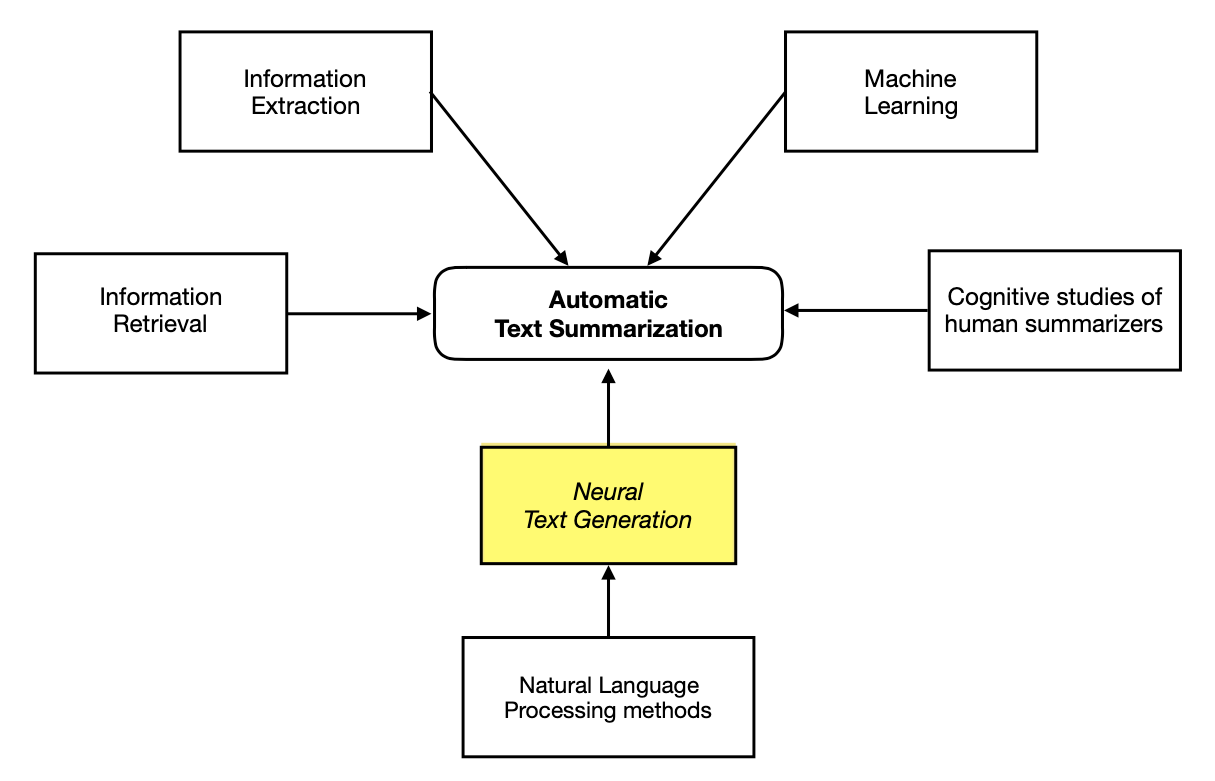
\includegraphics[width=5.5in]{photos/summ}\\
		\caption{Research fields with influence on the development of text summarization}\label{summ}
	\end{center}
\end{figure}

\begin{figure}
	\begin{center}
		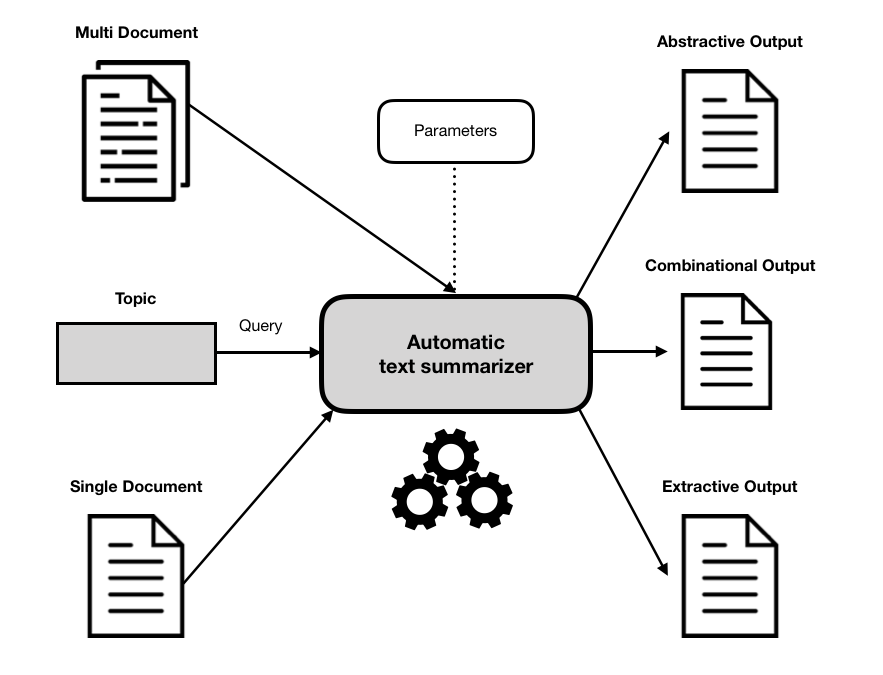
\includegraphics[width=5in]{photos/abex}\\
		\caption{Simplified Abstraction Extraction process}\label{abex}
	\end{center}
\end{figure}	

Figure \ref{abex} shows a simplified process of the abstractive or extractive approach. Both approaches can be applied decoupled from each other. The source documents, either single document or multi document go in as well with the topic of the topic (scientific, article, ...). The parameters are the compression rate \(\tau\), the type, etc. 

\subsubsection{Extractive}
\subsubsection{Abstractive}

\subsection{Evaluation}
ROGUE
BLEU


\section{Advanced Approaches for Text Summarization}\label{ss:trends}

\subsection{Combinational Approach}

\subsection{Reinforcement Learning}
